% ==============================================================================
% Projeto de Sistema - Gustavo Steim da Silveira
% Capítulo 4 - Arquitetura de Software
% ==============================================================================
\chapter{Arquitetura de Software}
\label{sec-arquitetura}
\vspace{-1cm} % Ajuste este espaçamento se necessário

O sistema \emph{\imprimirtitulo} foi desenvolvido seguindo a arquitetura clássica em camadas adotada por aplicações ASP.NET Core. Essa abordagem organiza a aplicação em módulos responsáveis por diferentes níveis de responsabilidade, promovendo a separação de interesses, reusabilidade e facilidade de manutenção.

\section{Visão Geral da Arquitetura em Camadas}

A Figura~\ref{figura-arquitetura-classica-dotnet} ilustra a arquitetura em camadas adotada no projeto. Essa estrutura compreende:

\begin{itemize}
    \item \textbf{Camada de Apresentação}: onde estão os controladores da API REST e, no frontend, os componentes Vue.js responsáveis pela interface com o usuário.
    \item \textbf{Camada de Aplicação}: que encapsula as regras de negócio por meio de serviços (Services) e objetos de transferência de dados (DTOs).
    \item \textbf{Camada de Domínio}: onde estão as entidades que representam os conceitos centrais do sistema.
    \item \textbf{Camada de Persistência}: que realiza o acesso ao banco de dados utilizando o Entity Framework Core.
\end{itemize}

\begin{figure}[H]
    \centering
    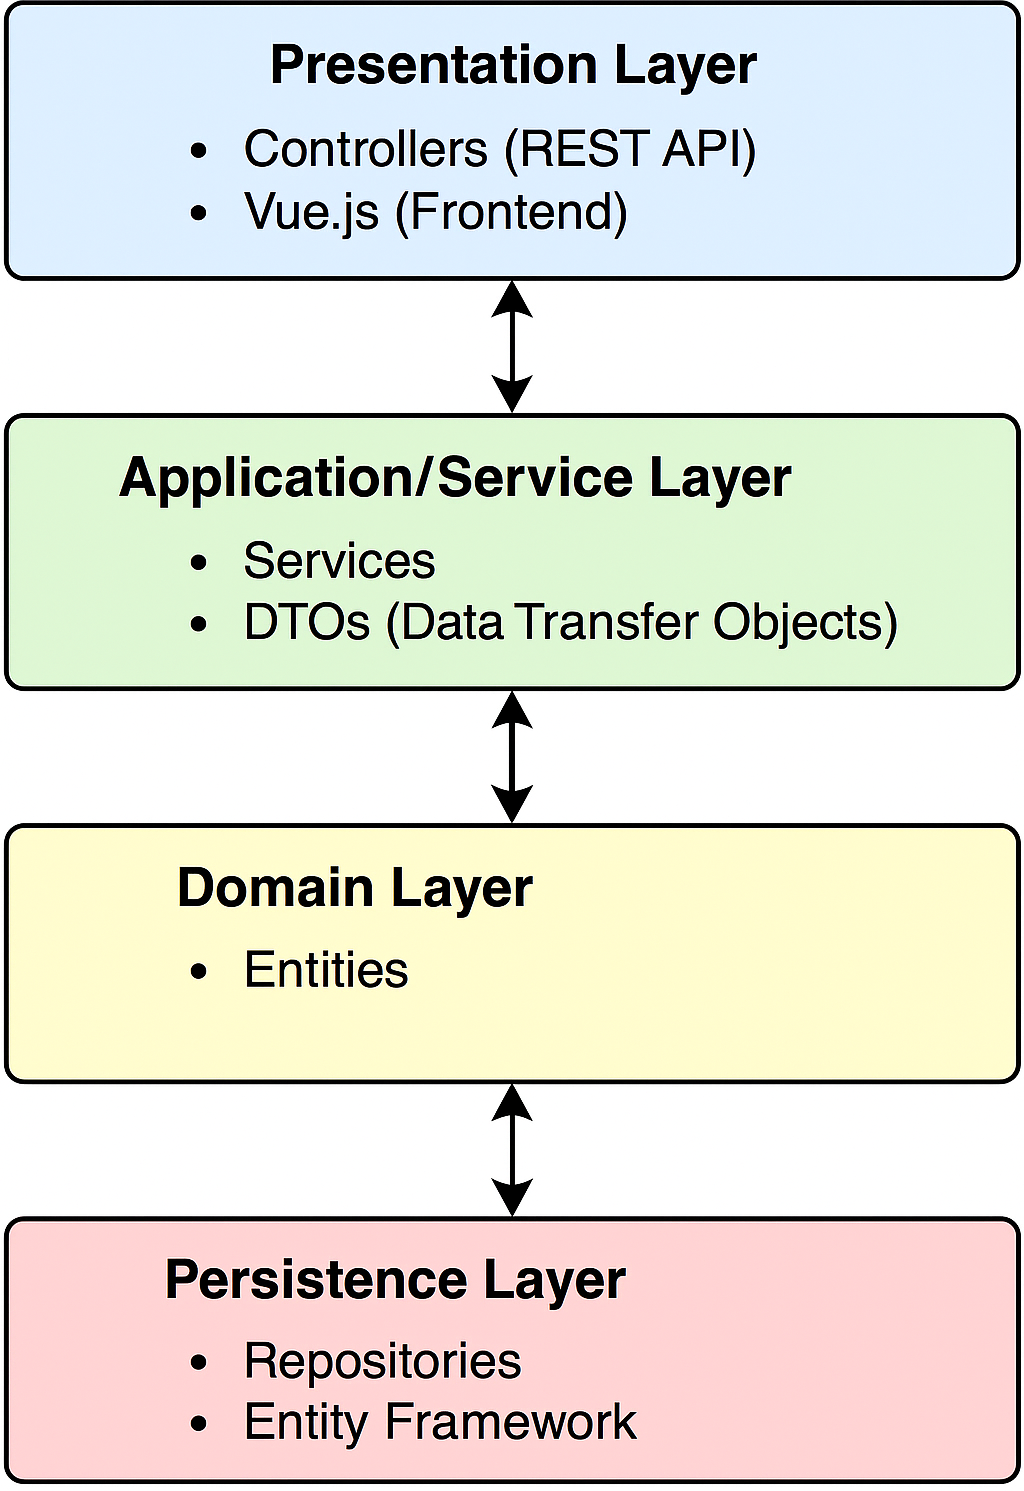
\includegraphics[width=0.9\textwidth]{figuras/arquitetura-dotnet-camadas.png}
    \caption{Arquitetura clássica em camadas do .NET}
    \label{figura-arquitetura-classica-dotnet}
\end{figure}

\section{Componentes do Sistema}

A seguir, apresentam-se os diagramas reais da implementação, agrupados conforme sua camada correspondente.

\subsection{Camada de Apresentação e Aplicação}

A Figura~\ref{figura-aplicacao} mostra os controladores e serviços responsáveis pelo fluxo da aplicação. As interfaces dos serviços (\textit{IUsuarioService}, \textit{IPerfilService}) são injetadas nos controladores seguindo o princípio de inversão de dependência.

\begin{figure}[H]
    \centering
    \includegraphics[width=\textwidth]{figuras/Aplicacao Class Diagram.png}
    \caption{Controladores, serviços e DTOs da aplicação}
    \label{figura-aplicacao}
\end{figure}

\subsection{Modelo de Domínio}

A Figura~\ref{figura-entidades} apresenta o modelo de entidades que representa os conceitos centrais do domínio, como usuários, perfis e permissões.

\begin{figure}[H]
    \centering
    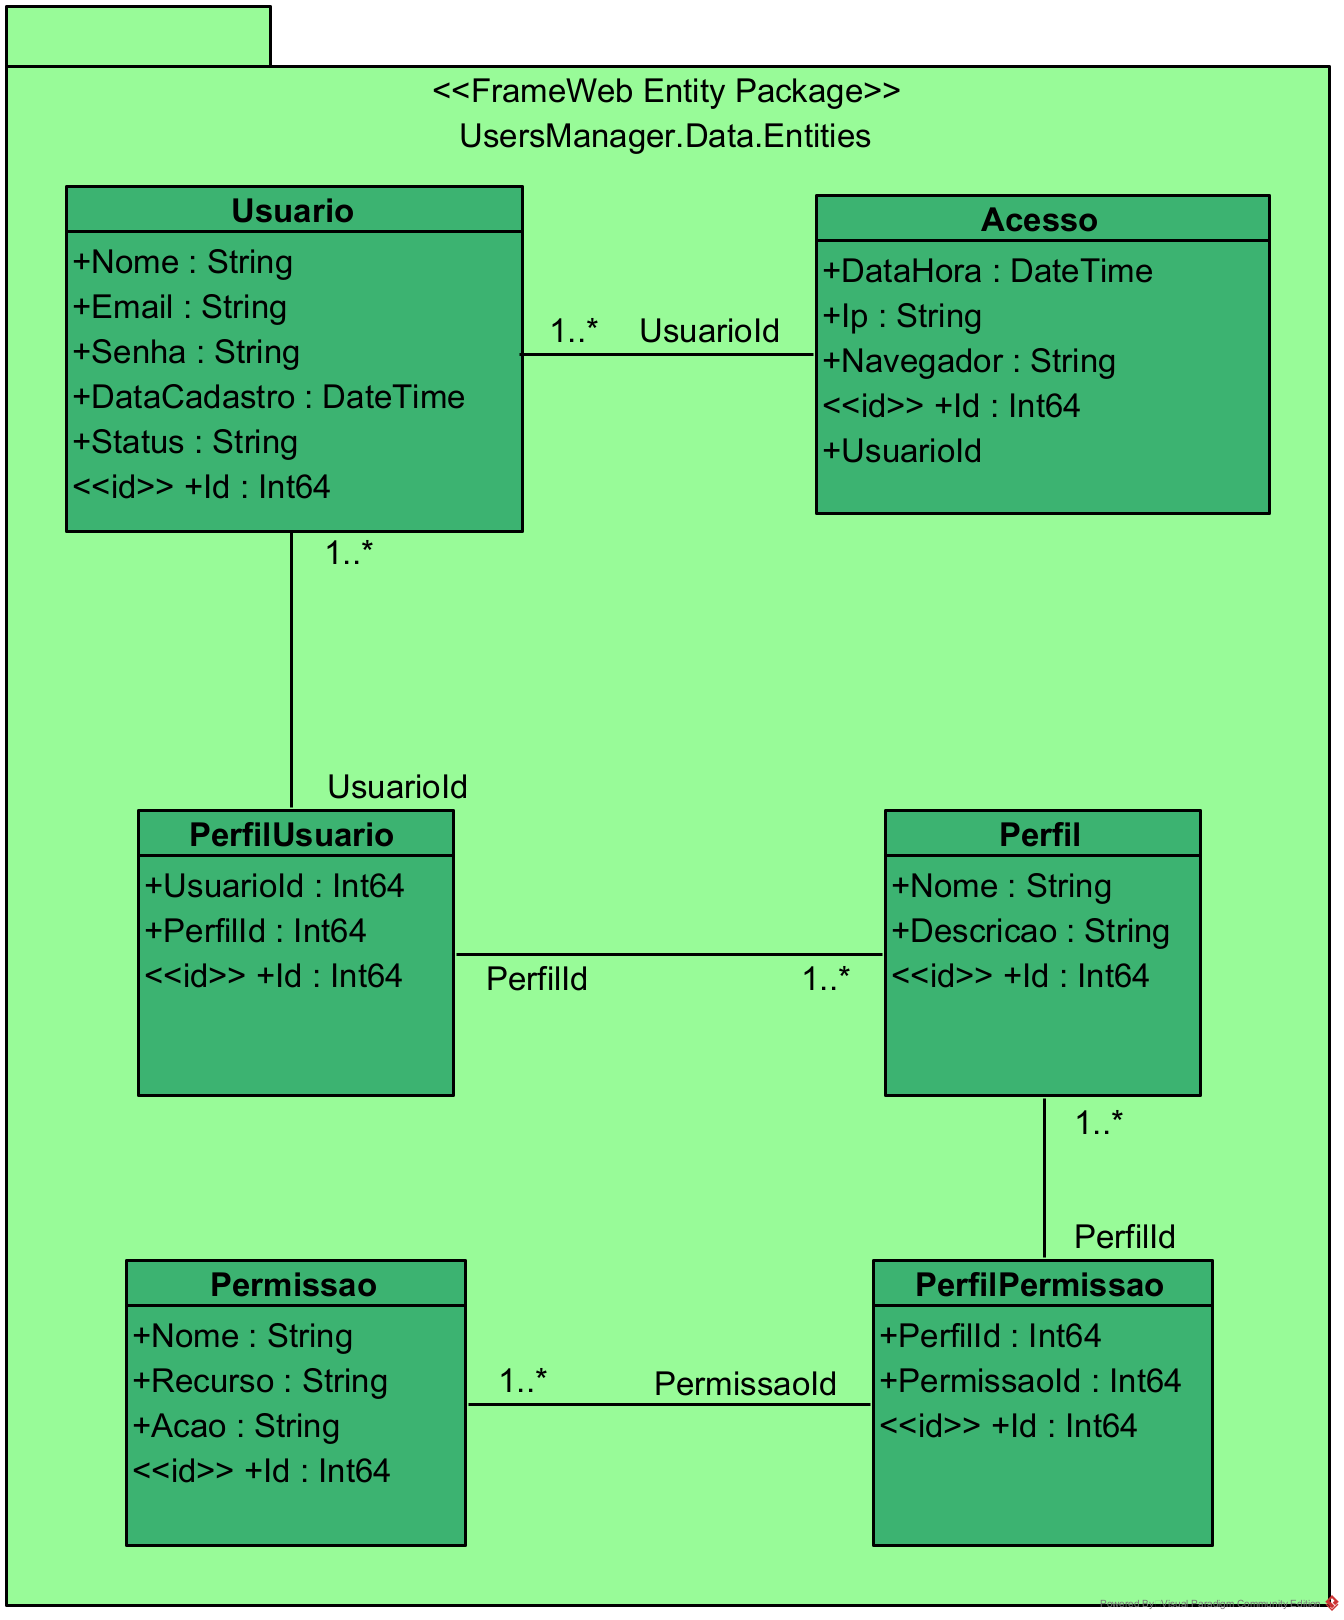
\includegraphics[width=0.8\textwidth]{figuras/Entidades Class Diagram.png}
    \caption{Entidades e relacionamentos do domínio}
    \label{figura-entidades}
\end{figure}

\subsection{Camada de Persistência}

A persistência é realizada via repositórios específicos para cada entidade, conforme ilustrado na Figura~\ref{figura-persistencia}. Esses componentes encapsulam as operações de consulta, inserção e atualização de dados utilizando o Entity Framework Core.

\begin{figure}[H]
    \centering
    \includegraphics[width=0.9\textwidth]{figuras/Persistencia Class Diagram.png}
    \caption{Repositórios e acesso a dados}
    \label{figura-persistencia}
\end{figure}

\section{Integração com o Frontend}

A comunicação entre o frontend Vue.js e o backend ASP.NET Core se dá por meio de requisições HTTP para a API RESTful. As figuras a seguir mostram os principais fluxos de navegação da aplicação:

\begin{itemize}
    \item Login: Figura~\ref{fig-navegacao-login}
    \item Edição de usuários: Figura~\ref{fig-navegacao-usuario}
    \item Gerenciamento de perfis: Figura~\ref{fig-navegacao-perfil}
    \item Dashboard: Figura~\ref{fig-navegacao-dashboard}
\end{itemize}

\begin{figure}[H]
    \centering
    \includegraphics[width=\textwidth]{figuras/Navegacao - Login.png}
    \caption{Navegação: processo de login}
    \label{fig-navegacao-login}
\end{figure}

\begin{figure}[H]
    \centering
    \includegraphics[width=\textwidth]{figuras/Navegacao - Edicao de Usuario.png}
    \caption{Navegação: edição de usuários}
    \label{fig-navegacao-usuario}
\end{figure}

\begin{figure}[H]
    \centering
    \includegraphics[width=\textwidth]{figuras/Navegacao - Edicao de Perfil.png}
    \caption{Navegação: gerenciamento de perfis e permissões}
    \label{fig-navegacao-perfil}
\end{figure}

\begin{figure}[H]
    \centering
    \includegraphics[width=\textwidth]{figuras/Navegacao - Ver Dashboard.png}
    \caption{Navegação: visualização do dashboard}
    \label{fig-navegacao-dashboard}
\end{figure}

\section{Considerações sobre Modelagem}

Embora o projeto utilize a arquitetura clássica do .NET, a modelagem inicial do sistema buscou inspiração em algumas diretrizes do FrameWeb, principalmente quanto à identificação de serviços e papéis das entidades no domínio. Para mais detalhes sobre a metodologia FrameWeb, consulte o projeto oficial\footnote{\url{https://nemo.inf.ufes.br/projetos/frameweb/}}.

% Referência ao FrameWeb (se usar bibtex ou manual)
% \bibitem{frameweb} Silva, C. A. et al. "FrameWeb: Uma abordagem orientada a modelos para aplicações Web baseadas em frameworks." Universidade Federal do Espírito Santo (UFES).

